\section{Results I: the compute-matched comparison}
\label{sec:results}

\subsection{CIFAR-10 with 10\% labels}
\label{sec:main}

\Cref{fig:budget} follows the four arms of the design from 970 to 97,000 steps under three protocols, and
\cref{tab:main} gives the numbers at four budgets. We first read the results with the oracle-label probe,
because it is the protocol used in most of the literature, and come back to the others in
\cref{sec:protocol}.

\begin{figure}[t]
\centering
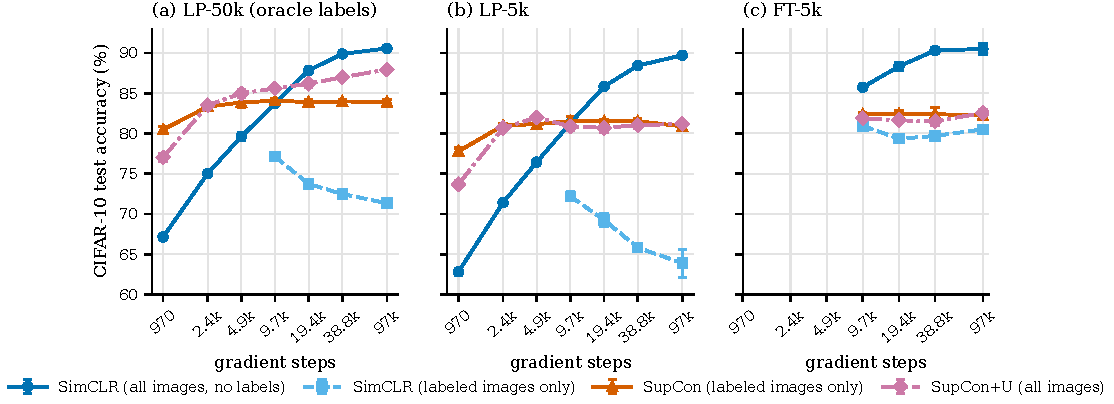
\includegraphics[width=\linewidth]{figures/fig_budget.pdf}
\caption{CIFAR-10, 10\% labels, ResNet-18: test accuracy against the number of gradient steps for the four
arms of the $2\times2$ design. Mean and standard deviation over seeds (five at 9,700 and 19,400 steps,
three elsewhere). (a) With the oracle-label probe, \supcon is far ahead early, level with \simclr at 9,700
steps and behind afterwards. (b, c) With the 5,000 labels only, \simclr is ahead of both label-using methods
from 9,700 steps on. Fine-tuning was run from 9,700 steps on.}
\label{fig:budget}
\end{figure}

\begin{table}[t]
\centering
\small
\caption{CIFAR-10, 10\% labels, ResNet-18. Test accuracy (\%), mean $\pm$ standard deviation over seeds;
best mean per budget and column in bold. \lpall and $k$NN-50k use all 50,000 labels; \lpfive and \ftfive use
only the 5,000 labels of the budget. All budgets are listed in \cref{tab:budgets}; tests are in
\cref{tab:stats}.}
\label{tab:main}
% generated by scripts/make_assets.py -- do not edit
\begin{tabular}{lccccc}
\toprule
 & & \multicolumn{2}{c}{oracle labels (50k)} & \multicolumn{2}{c}{label budget (5k)} \\
\cmidrule(lr){3-4}\cmidrule(lr){5-6}
method & seeds & LP-50k & $k$NN-50k & LP-5k & FT-5k \\
\midrule
\multicolumn{6}{l}{\emph{9,700 steps}} \\
\quad \simclrsub & 5 & 77.1{\scriptsize$\,\pm\,$0.4} & 74.0{\scriptsize$\,\pm\,$0.3} & 72.2{\scriptsize$\,\pm\,$0.5} & 81.0{\scriptsize$\,\pm\,$0.4} \\
\quad \simclr & 5 & 83.7{\scriptsize$\,\pm\,$0.2} & 79.8{\scriptsize$\,\pm\,$0.2} & 81.3{\scriptsize$\,\pm\,$0.2} & \textbf{85.9}{\scriptsize$\,\pm\,$0.4} \\
\quad \supcon & 5 & 84.1{\scriptsize$\,\pm\,$0.3} & 82.2{\scriptsize$\,\pm\,$0.4} & \textbf{81.5}{\scriptsize$\,\pm\,$0.5} & 82.3{\scriptsize$\,\pm\,$0.1} \\
\quad \union & 5 & \textbf{85.6}{\scriptsize$\,\pm\,$0.1} & \textbf{83.2}{\scriptsize$\,\pm\,$0.3} & 80.9{\scriptsize$\,\pm\,$0.5} & 81.9{\scriptsize$\,\pm\,$0.4} \\
\multicolumn{6}{l}{\emph{19,400 steps}} \\
\quad \simclrsub & 5 & 73.7{\scriptsize$\,\pm\,$0.2} & 71.2{\scriptsize$\,\pm\,$0.3} & 69.2{\scriptsize$\,\pm\,$0.9} & -- \\
\quad \simclr & 5 & \textbf{87.8}{\scriptsize$\,\pm\,$0.2} & \textbf{85.7}{\scriptsize$\,\pm\,$0.3} & \textbf{85.8}{\scriptsize$\,\pm\,$0.2} & \textbf{88.6}{\scriptsize$\,\pm\,$0.4} \\
\quad \supcon & 5 & 83.9{\scriptsize$\,\pm\,$0.3} & 82.4{\scriptsize$\,\pm\,$0.1} & 81.5{\scriptsize$\,\pm\,$0.3} & 82.2{\scriptsize$\,\pm\,$0.2} \\
\quad \union & 5 & 86.2{\scriptsize$\,\pm\,$0.4} & 84.3{\scriptsize$\,\pm\,$0.3} & 80.7{\scriptsize$\,\pm\,$0.6} & 81.7{\scriptsize$\,\pm\,$0.3} \\
\bottomrule
\end{tabular}

\end{table}

\paragraph{Labels buy speed}
After 970 steps \supcon reaches \R{supcon_lab_f0.1_e10:lp50:pm}\% and \simclr \R{simclr_all_e10:lp50:pm}\%, a
gap of \R{d:simclr-supcon:lp50:e10}\pt in favour of the method that uses labels. The gap shrinks to
\R{d:simclr-supcon:lp50:e25}\pt at 2,425 steps and \R{d:simclr-supcon:lp50:e50}\pt at 4,850. At 9,700 steps the
two are level: the difference is \R{cmp:simclr-supcon:lp50:e100:sdiff}\pt (95\% interval
\R{cmp:simclr-supcon:lp50:e100:ci}), and the equivalence test accepts a margin of $\pm1$ point
($p=\R{cmp:simclr-supcon:lp50:e100:tost}$). This agrees with SuNCEt \citep{assran2020suncet}: labels in the
loss reach a given accuracy with much less compute.

\paragraph{The lead does not last}
\supcon stops improving early, because once its 5,000 images are separated by class the loss has little
left to learn from them (\cref{sec:geometry}). It is at \R{supcon_lab_f0.1_e25:lp50}\% after 2,425 steps, \R{supcon_lab_f0.1_e200:lp50}\% after 19,400 and
\R{supcon_lab_f0.1_e400:lp50}\% after 38,800. \simclr keeps climbing: \R{simclr_all_e100:lp50}\% at 9,700 steps,
\R{simclr_all_e200:lp50}\% at 19,400 and \R{simclr_all_e400:lp50}\% at 38,800. It is ahead by
\R{cmp:simclr-supcon:lp50:e200:diff}\pt at 19,400 steps (\R{cmp:simclr-supcon:lp50:e200:ci},
$p\,\R{cmp:simclr-supcon:lp50:e200:p}$ after correction) and by \R{cmp:simclr-supcon:lp50:e400:diff}\pt at
38,800 (\R{cmp:simclr-supcon:lp50:e400:ci}). The crossover is therefore not an artefact of a short budget: it
widens as training gets longer. At 97,000 steps \supcon is still at \R{supcon_lab_f0.1_e1000:lp50}\% and
\simclr reaches \R{simclr_all_e1000:lp50}\%, a lead of \R{cmp:simclr-supcon:lp50:e1000:diff}\pt
(\R{cmp:simclr-supcon:lp50:e1000:ci}); after fine-tuning on the 5,000 labels the lead is
\R{cmp:simclr-supcon:ft:e1000:diff}\pt (\R{simclr_all_e1000:ft}\% against \R{supcon_lab_f0.1_e1000:ft}\%,
\R{cmp:simclr-supcon:ft:e1000:ci}). \union, which also sees all images, keeps improving too (\R{union_f0.1_e400:lp50}\% at 38,800
steps and \R{union_f0.1_e1000:lp50}\% at 97,000), because three quarters of each of its batches are unlabeled
images trained by instance discrimination; it stays \R{d:simclr-union:lp50:e1000}\pt behind \simclr.

\paragraph{Reading the $2\times2$}
The two columns of the design answer what the unlabeled images are worth. Without labels the answer is
``a lot, and more with time'': \simclr on all images beats \simclr on the labeled subset by
\R{cmp:simclr-sub:lp50:e100:diff}\pt at 9,700 steps and by \R{cmp:simclr-sub:lp50:e200:diff}\pt at 19,400,
because \simclrsub gets \emph{worse} with more steps (\R{simclr_sub_f0.1_e100:lp50}\% $\to$
\R{simclr_sub_f0.1_e200:lp50}\% $\to$ \R{simclr_sub_f0.1_e1000:lp50}\% at 97,000 steps). With 5,000 images, each one returns in every tenth batch, and instance
discrimination can then be solved with features that identify individual images rather than features shared
within a class: more steps lower the loss on the pool without improving the representation. With labels the unlabeled
images help less: \union beats \supcon by \R{cmp:union-supcon:lp50:e100:diff}\pt and
\R{cmp:union-supcon:lp50:e200:diff}\pt.

The two rows answer what the labels are worth. On the small pool they are worth a great deal: \supcon beats
\simclrsub by \R{cmp:supcon-sub:lp50:e100:diff}\pt at 9,700 steps. On the full pool the answer depends on the
budget: \union is \R{d:simclr-union:lp50:e100}\pt ahead of \simclr at 9,700 steps and
\R{d:simclr-union:lp50:e200}\pt behind at 19,400. So under the oracle-label probe, adding labels to a
contrastive loss that already sees all images helps for short budgets only, and adding unlabeled images to
\supcon always helps a little. \Cref{sec:protocol} shows that the second statement does not survive a change
of protocol.

\subsection{Is the plateau of \supcon a tuning failure?}
\label{sec:plateau}
A plateau after a few thousand steps on 5,000 images could simply mean that \supcon is under-regularised:
9,700 steps are almost a thousand passes over the labeled images. We tested four explanations.

\emph{Temperature.} The rows of the design differ in temperature. Swapping them does not help either
method: \simclr with $\tau=0.1$ reaches \R{simclr_all_t0.1_e100:lp50}\% (default
\R{simclr_all_e100:lp50}\%) and \supcon with $\tau=0.5$ reaches \R{supcon_lab_f0.1_t0.5_e100:lp50}\% (default
\R{supcon_lab_f0.1_e100:lp50}\%) at 9,700 steps (one seed each). A low temperature makes \simclr
concentrate on its most similar negatives, which are often images of the same class, and push them apart;
a high temperature weakens the class-level attraction that \supcon gets from its labels.

\emph{Weight decay and augmentation.} \pending{At 38,800 steps we raised the weight decay of \supcon from
$10^{-4}$ to $5\times10^{-4}$ and $10^{-3}$, strengthened the augmentation (crop scale 0.08--1 and
full-strength colour jitter), and combined both (\cref{tab:reg}). The best variant reaches
\R{reg:best}\%, against \R{supcon_lab_f0.1_e400:lp50}\% for the default.}

\emph{Early stopping.} The best checkpoint along the longest \supcon run, selected with all 50,000 labels and
therefore an upper bound on any early-stopping rule, reaches \R{bestknn:supcon}\% $k$NN accuracy, against
\R{bestknn:simclr}\% for \simclr.

\emph{Learning-rate schedule.} Every budget is a separate run with its own warm-up and cosine schedule, so
no point of \cref{fig:budget} is a truncated longer run.

None of these changes the conclusion that, with 5,000 labeled images, \supcon saturates several points below
where label-free pretraining on all images arrives.

\subsection{Label fraction and budget together}
\label{sec:fractions}
\Cref{fig:wins} extends the comparison to label fractions from 1\% to 100\% and to three budgets. Each cell
is the accuracy of the label-using method minus that of \simclr at the same number of steps, under the
all-label probe (LP-all) and under a probe that sees only the fraction $f$ of the labels (LP-$f$).

\begin{figure}[t]
\centering
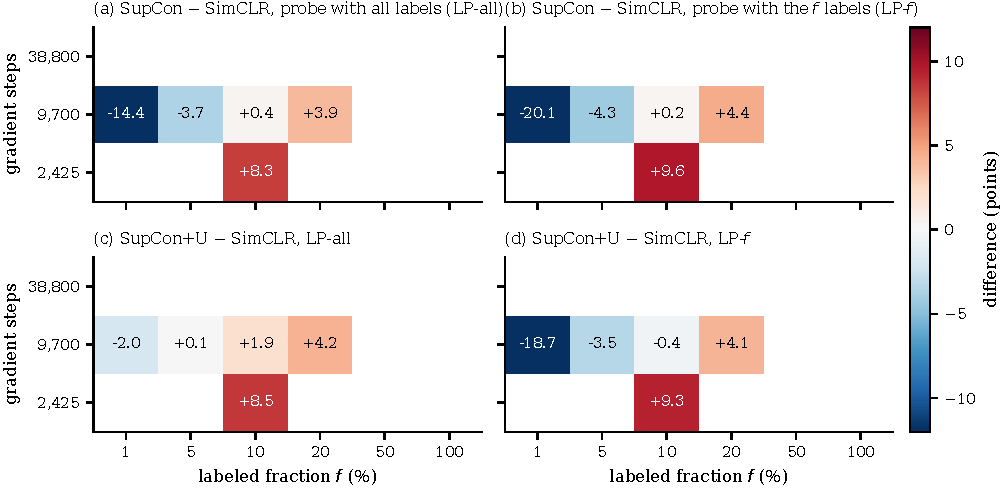
\includegraphics[width=\linewidth]{figures/fig_wins.pdf}
\caption{Which method wins, by label fraction and budget (CIFAR-10, ResNet-18, one seed except $f=10\%$).
Cells show the accuracy of \supcon (a, b) or \union (c, d) minus that of \simclr at the same number of steps;
red means that the label-using method is ahead. LP-all is the oracle-label probe; LP-$f$ uses the same
fraction of labels as pretraining. The numbers behind the chart are in \cref{tab:fraction}.}
\label{fig:wins}
\end{figure}

\pending{Three regions are visible. With few labels and many steps (upper left) \simclr wins under both
probes. With many labels (right) \supcon wins everywhere, in line with the full-label result of
\citet{khosla2020supcon}; the break-even fraction moves to the right as the budget grows. With few steps
(bottom row) the label-using methods win at every fraction, the speed effect of \cref{sec:main}. The LP-$f$
panels are shifted towards \simclr relative to the LP-all panels, most strongly for \union, which is the
protocol effect studied in \cref{sec:protocol}.}

\subsection{Other datasets and a larger encoder}
\label{sec:datasets}

\begin{table}[t]
\centering
\small
\caption{The four arms on CIFAR-100, on STL-10 and with a ResNet-50 (test accuracy in \%, mean $\pm$
standard deviation over seeds). LP-all uses all training labels and is not available on STL-10, whose
5,000 labels are the whole labeled set; LP-budget and FT-budget use the labels of the budget only.}
\label{tab:datasets}
\begin{adjustbox}{max width=\linewidth}
% generated by scripts/make_assets.py -- do not edit
\begin{tabular}{lrcccc}
\toprule
method & steps & seeds & LP-all & LP-budget & FT-budget \\
\midrule
\multicolumn{6}{l}{\emph{CIFAR-100, 10\% labels (5,000), ResNet-18}} \\
\quad \simclrsub & 9,700 & 3 & 44.5{\scriptsize$\,\pm\,$0.2} & 33.0{\scriptsize$\,\pm\,$0.1} & 42.6{\scriptsize$\,\pm\,$0.3} \\
\quad \simclr & 9,700 & 3 & 54.6{\scriptsize$\,\pm\,$0.4} & 43.5{\scriptsize$\,\pm\,$0.3} & \textbf{50.7}{\scriptsize$\,\pm\,$1.3} \\
\quad \supcon & 9,700 & 3 & 51.0{\scriptsize$\,\pm\,$0.7} & 41.8{\scriptsize$\,\pm\,$0.8} & 44.4{\scriptsize$\,\pm\,$0.6} \\
\quad \union & 9,700 & 3 & \textbf{56.1}{\scriptsize$\,\pm\,$0.7} & \textbf{44.9}{\scriptsize$\,\pm\,$0.2} & 47.7{\scriptsize$\,\pm\,$1.1} \\
\quad \simclr & 19,400 & 3 & \textbf{59.5}{\scriptsize$\,\pm\,$0.2} & \textbf{51.0}{\scriptsize$\,\pm\,$0.4} & \textbf{55.1}{\scriptsize$\,\pm\,$0.8} \\
\quad \supcon & 19,400 & 3 & 50.2{\scriptsize$\,\pm\,$0.2} & 40.3{\scriptsize$\,\pm\,$0.5} & 43.0{\scriptsize$\,\pm\,$0.7} \\
\quad \union & 19,400 & 3 & 57.5{\scriptsize$\,\pm\,$0.5} & 41.3{\scriptsize$\,\pm\,$0.5} & 43.7{\scriptsize$\,\pm\,$0.7} \\
\addlinespace
\multicolumn{6}{l}{\emph{STL-10, 5,000 labels + 100,000 unlabeled images, 96 px, ResNet-18}} \\
\quad \simclrsub & 20,500 & 3 & -- & 70.9{\scriptsize$\,\pm\,$0.4} & 82.3{\scriptsize$\,\pm\,$0.4} \\
\quad \simclr & 20,500 & 3 & -- & \textbf{84.4}{\scriptsize$\,\pm\,$0.7} & \textbf{89.4}{\scriptsize$\,\pm\,$0.4} \\
\quad \supcon & 20,500 & 3 & -- & 83.8{\scriptsize$\,\pm\,$0.2} & 84.1{\scriptsize$\,\pm\,$0.3} \\
\quad \union & 20,500 & 3 & -- & 83.7{\scriptsize$\,\pm\,$0.4} & 83.5{\scriptsize$\,\pm\,$0.4} \\
\quad \simclrsub & 41,000 & 3 & -- & 69.3{\scriptsize$\,\pm\,$0.4} & 82.6{\scriptsize$\,\pm\,$0.3} \\
\quad \simclr & 41,000 & 3 & -- & \textbf{86.9}{\scriptsize$\,\pm\,$1.1} & \textbf{90.8}{\scriptsize$\,\pm\,$0.2} \\
\quad \supcon & 41,000 & 3 & -- & 83.9{\scriptsize$\,\pm\,$0.6} & 84.5{\scriptsize$\,\pm\,$0.4} \\
\quad \union & 41,000 & 3 & -- & 84.3{\scriptsize$\,\pm\,$0.6} & 84.2{\scriptsize$\,\pm\,$0.4} \\
\addlinespace
\multicolumn{6}{l}{\emph{Tiny-ImageNet, 10\% labels (10,000), 64 px, ResNet-18}} \\
\quad \simclrsub & 19,500 & 3 & 24.4{\scriptsize$\,\pm\,$0.2} & 16.8{\scriptsize$\,\pm\,$0.4} & 26.7{\scriptsize$\,\pm\,$1.3} \\
\quad \simclr & 19,500 & 3 & 37.8{\scriptsize$\,\pm\,$0.4} & 28.5{\scriptsize$\,\pm\,$0.3} & \textbf{35.3}{\scriptsize$\,\pm\,$0.3} \\
\quad \supcon & 19,500 & 3 & 35.6{\scriptsize$\,\pm\,$0.2} & 26.6{\scriptsize$\,\pm\,$0.2} & 28.6{\scriptsize$\,\pm\,$1.0} \\
\quad \union & 19,500 & 3 & \textbf{40.2}{\scriptsize$\,\pm\,$0.2} & \textbf{28.9}{\scriptsize$\,\pm\,$0.3} & 33.6{\scriptsize$\,\pm\,$0.4} \\
\quad \simclrsub & 39,000 & 3 & 21.8{\scriptsize$\,\pm\,$0.1} & 14.2{\scriptsize$\,\pm\,$0.2} & 26.2{\scriptsize$\,\pm\,$0.5} \\
\quad \simclr & 39,000 & 3 & \textbf{42.1}{\scriptsize$\,\pm\,$0.2} & \textbf{33.2}{\scriptsize$\,\pm\,$0.4} & \textbf{37.3}{\scriptsize$\,\pm\,$0.2} \\
\quad \supcon & 39,000 & 3 & 35.3{\scriptsize$\,\pm\,$0.2} & 26.4{\scriptsize$\,\pm\,$0.4} & 28.4{\scriptsize$\,\pm\,$0.1} \\
\quad \union & 39,000 & 3 & 39.5{\scriptsize$\,\pm\,$0.2} & 21.5{\scriptsize$\,\pm\,$1.0} & 30.3{\scriptsize$\,\pm\,$0.9} \\
\addlinespace
\multicolumn{6}{l}{\emph{CIFAR-10, 10\% labels, ResNet-50}} \\
\quad \simclr & 9,700 & 1 & 85.8 & 82.6 & \textbf{85.6} \\
\quad \supcon & 9,700 & 1 & 86.4 & \textbf{82.9} & 83.6 \\
\quad \union & 9,700 & 1 & \textbf{87.2} & 81.2 & 82.4 \\
\quad \simclr & 19,400 & 3 & \textbf{90.0}{\scriptsize$\,\pm\,$0.1} & \textbf{87.8}{\scriptsize$\,\pm\,$0.1} & \textbf{89.4}{\scriptsize$\,\pm\,$0.3} \\
\quad \supcon & 19,400 & 3 & 85.7{\scriptsize$\,\pm\,$0.2} & 82.5{\scriptsize$\,\pm\,$0.2} & 83.2{\scriptsize$\,\pm\,$0.1} \\
\bottomrule
\end{tabular}

\end{adjustbox}
\end{table}

\paragraph{CIFAR-100}
With 10\% labels there are 50 labeled images per class (three seeds). At 9,700 steps \union is the best arm
under the oracle-label probe (\R{c100_union_f0.1_e100:lp50}\%), ahead of \simclr
(\R{c100_simclr_all_e100:lp50}\%) and \supcon (\R{c100_supcon_lab_f0.1_e100:lp50}\%), and it is still first with
\lpfive (\R{c100_union_f0.1_e100:lp5}\% against \R{c100_simclr_all_e100:lp5}\%). After fine-tuning on the 5,000
labels the order is \simclr (\R{c100_simclr_all_e100:ft}\%), \union (\R{c100_union_f0.1_e100:ft}\%), \supcon
(\R{c100_supcon_lab_f0.1_e100:ft}\%). That \lpfive does not yet reverse the order matches CIFAR-10, where at
9,700 steps \simclr and \union are also within a point under \lpfive (\cref{tab:main}): \simclr is still far
from its end point at this budget, and the gap opens only with longer training. \pending{CIFAR-100 at 19,400
steps is in progress.}

\paragraph{STL-10}
STL-10 has no oracle labels, so every protocol uses its 5,000 labels, and its 100,000 unlabeled images are
not restricted to the ten classes. At 20,500 steps, about 100 passes over the 105,000 images and therefore
the counterpart of 9,700 steps on CIFAR, the linear probe does not separate the three arms: \simclr reaches
\R{stl_simclr_all_e100:lp5:pm}\%, \supcon \R{stl_supcon_lab_e100:lp5:pm}\% and \union
\R{stl_union_e100:lp5:pm}\%. The differences, \R{cmp:stl:simclr-supcon:lp50:e100:sdiff}\pt
(\R{cmp:stl:simclr-supcon:lp50:e100:ci}) and \R{cmp:stl:simclr-union:lp50:e100:sdiff}\pt
(\R{cmp:stl:simclr-union:lp50:e100:ci}), are not significant, as on CIFAR-10 at the same number of passes;
the intervals are still too wide to claim equivalence within one point. Fine-tuning
separates them clearly: \simclr reaches \R{stl_simclr_all_e100:ft:pm}\%, \R{cmp:stl:simclr-supcon:ft:e100:diff}\pt
above \supcon (\R{cmp:stl:simclr-supcon:ft:e100:ci}) and \R{cmp:stl:simclr-union:ft:e100:diff}\pt above \union.
$k$NN on the 5,000 labels favours the label-using encoders (\R{stl_supcon_lab_e100:knn}\% against
\R{stl_simclr_all_e100:knn}\% for \simclr), because a nearest-neighbour rule works best when the labeled
images form tight clusters, which is what \supcon makes of them. The seen/unseen gap of
\cref{sec:geometry} appears here too: the CDNV of \supcon is \R{stl_supcon_lab_e100:cdnv_lab} on its labeled
images and \R{stl_supcon_lab_e100:cdnv_test} on test images, against \R{stl_simclr_all_e100:cdnv_lab} and
\R{stl_simclr_all_e100:cdnv_test} for \simclr. The unlabeled images are worth
\R{cmp:stl:simclr-sub:lp50:e100:diff}\pt of \lpfive to \simclr (\simclrsub reaches
\R{stl_simclr_sub_e100:lp5}\%), although many of them show other classes. For reference, cross-entropy on the
5,000 labels reaches \R{stl_ce_e100:clf:pm}\% and FixMatch \R{stl_fixmatch:clf:pm}\%.
At 41,000 steps the crossover of \cref{sec:main} appears on STL-10 as well. \supcon and \union barely move
(\R{stl_supcon_lab_e200:lp5:pm}\% and \R{stl_union_e200:lp5:pm}\% with \lpfive), for the same reason as on
CIFAR-10: their 5,000 labeled images are already separated by class. \simclr climbs to
\R{stl_simclr_all_e200:lp5:pm}\%, \R{cmp:stl:simclr-supcon:lp50:e200:diff}\pt above \supcon
(\R{cmp:stl:simclr-supcon:lp50:e200:ci}) and \R{cmp:stl:simclr-union:lp50:e200:diff}\pt above \union
(\R{cmp:stl:simclr-union:lp50:e200:ci}). After fine-tuning its lead grows to
\R{cmp:stl:simclr-supcon:ft:e200:diff}\pt and \R{cmp:stl:simclr-union:ft:e200:diff}\pt
(\R{stl_simclr_all_e200:ft:pm}\%), and the $k$NN advantage of the label-using encoders is gone
(\R{stl_simclr_all_e200:knn}\% for \simclr against \R{stl_supcon_lab_e200:knn}\% for \supcon).
\pending{(FixMatch from these encoders is in progress.)}

\paragraph{ResNet-50}
With a ResNet-50 the crossover under the oracle-label probe comes later than with a ResNet-18, as expected
from the finding that label-free contrastive learning gains more than supervised training from larger
encoders and longer training \citep{chen2020simclr}. At 9,700
steps \supcon is still slightly ahead (\R{r50_supcon_lab_f0.1_e100:lp50}\% against
\R{r50_simclr_all_e100:lp50}\%, one seed); at 19,400 steps \simclr is clearly ahead
(\R{r50_simclr_all_e200:lp50}\% against \R{r50_supcon_lab_f0.1_e200:lp50}\%; \pending{one seed, two more in
progress}). Under \ftfive
\simclr is ahead already at 9,700 steps (\R{r50_simclr_all_e100:ft}\% against
\R{r50_supcon_lab_f0.1_e100:ft}\%). The larger encoder also makes very short budgets fragile: at 900 steps
\supcon reaches \R{r50_supcon_lab_f0.1_steps900:lp50}\% with learning rate 0.25 but only
\R{r50_supcon_lab_f0.1_steps900_lr0.05:lp50}\% with 0.05 (\cref{tab:r50}): with so few steps and a cosine
schedule, the smaller learning rate leaves the larger network far from convergence.
